\documentclass[11pt,a4paper]{article}

\usepackage[margin=2.2cm]{geometry}
\usepackage{amsmath,amssymb}
\usepackage{booktabs}
\usepackage{graphicx}
\usepackage{caption}
\usepackage{float}
\usepackage{siunitx}
\DeclareSIUnit{\GeV}{\giga\electronvolt}
\DeclareSIUnit{\keV}{\kilo\electronvolt}
\DeclareSIUnit{\ns}{\nano\second}
\DeclareSIUnit{\cm}{\centi\metre}
\DeclareSIUnit{\mm}{\milli\metre}
\DeclareSIUnit{\rad}{\radian}
\usepackage[hidelinks]{hyperref}
\usepackage{microtype}
\usepackage{setspace}
\setstretch{1.08}

\graphicspath{{../figures/}}

\title{Quirk plane search:\\ efficiencies, uncertainties, and Figures 2--5}
\author{Comparison with Knapen, Lou, Papucci, and Setford, arXiv:1708.02243}
\date{}

\begin{document}
\maketitle

\begin{abstract}
This note reports a 2000-event electroweak sample and a 2000-event colored sample of the quirk plane search.
Every cut is counted sequentially.
Each efficiency is given with its binomial standard error and a Wilson 95\% confidence interval, and is compared with Table~I of the paper.
Figures~2--5 of the paper are reproduced for these benchmarks: the internal angular momentum and separation, the rotation of the quirk plane, one event projected onto its reconstructed plane, and the distributions of the thickness \(\Delta s\) and the width \(\Delta w\).
\end{abstract}

\section{Samples}
Both samples use the straight-string equation of motion, a \SI{2}{\tesla} solenoid, and the eight-layer barrel.
The electroweak sample has mass \(m_Q = \SI{800}{\GeV}\).
The colored sample has mass \(m_Q = \SI{1800}{\GeV}\).
Both use the string scale \(\Lambda = \SI{4}{\keV}\).
Each sample contains \(N_{\mathrm{gen}} = 2000\) events, generated on 16 cores.
The four-momenta come from the built-in sampler.
MadGraph and Pythia were not used.

\section{Efficiency definitions}
An event is counted at a cut only if it has passed every earlier cut.
The three efficiencies in the paper are ratios of those counts,
\begin{align}
\varepsilon_{\mathrm{trig}}
  &= \frac{N_{\mathrm{trig}}}{N_{\mathrm{gen}}},
  &
  N_{\mathrm{trig}}
  &= \#\{p_T > \SI{200}{\GeV}\},
  \label{eq:trig}
  \\
\varepsilon_{\mathrm{fid}}
  &= \frac{N_{\mathrm{fid}}}{N_{\mathrm{trig}}},
  \label{eq:fid}
  \\
\varepsilon_{\mathrm{reco}}
  &= \frac{N_{\mathrm{reco}}}{N_{\mathrm{fid}}},
  \label{eq:reco}
  \\
\varepsilon
  &= \varepsilon_{\mathrm{trig}}\,
     \varepsilon_{\mathrm{fid}}\,
     \varepsilon_{\mathrm{reco}}
   = \frac{N_{\mathrm{reco}}}{N_{\mathrm{gen}}}.
  \label{eq:total}
\end{align}
The fiducial count \(N_{\mathrm{fid}}\) requires both quirks to intersect all eight barrel layers, with every hit time below \SI{25}{\ns}.
The reconstruction count \(N_{\mathrm{reco}}\) is the number of events that pass the final hit-pattern cut.
Because the flow is sequential, that count already requires the trigger, the fiducial requirement, the seed windows, the factor-of-three growth test, \(\Delta w < \SI{1}{\cm}\), and \(\Delta s < \SI{0.01}{\cm}\).

The individual cuts, in order, are:
\begin{enumerate}
\item \textbf{Generated.} Every simulated event.
\item \textbf{Trigger.} Pair transverse momentum above \SI{200}{\GeV}.
\item \textbf{Fiducial.} Both quirks hit all eight layers within \SI{25}{\ns}.
\item \textbf{Layer-8 seed.} A hit pair on layer 8 with \(\Delta\phi < 0.1\) and \(\Delta z < \SI{2}{\cm}\).
\item \textbf{Layer-7 seed.} A hit pair on layer 7 in the same window.
\item \textbf{Seed prefilter.} The two pairs agree within \SI{0.5}{\rad} and \SI{80}{\mm}. This removes combinations that cannot satisfy the \SI{1}{\cm} width cut.
\item \textbf{Seed thickness.} The four seed hits have \(\Delta s < \SI{0.05}{\cm}\).
\item \textbf{Seed width.} The four seed hits have \(\Delta w < \SI{1}{\cm}\).
\item \textbf{Forward direction.} Every seed hit satisfies \(\boldsymbol{n}_3\cdot\boldsymbol{x} > 0\).
\item \textbf{Inward walk.} From layer 6 down to layer 1, a hit is added only when both \(\Delta s\) and \(\Delta w\) stay within a factor of three of their current values, and the finished plane has \(\Delta w < \SI{1}{\cm}\).
\item \textbf{Final thickness.} The finished plane has \(\Delta s < \SI{0.01}{\cm}\).
\item \textbf{Hit pattern.} Seven layers contain two hits and the remaining layer contains at least one.
\end{enumerate}

\section{Wilson intervals}
Each efficiency is a binomial proportion \(k/n\), with estimate \(\hat{p} = k/n\).
The standard error is
\begin{equation}
\sigma = \sqrt{\frac{\hat{p}\,(1-\hat{p})}{n}}.
\label{eq:se}
\end{equation}
The 95\% interval is the Wilson score interval. With \(z = 1.960\),
\begin{equation}
\begin{aligned}
\hat{p}_{\mathrm{W}}
&=
\left(\hat{p} + \frac{z^{2}}{2n}\right)
\frac{1}{1 + z^{2}/n},
\\
\delta
&=
\frac{z}{1 + z^{2}/n}
\sqrt{
  \frac{\hat{p}\,(1-\hat{p})}{n}
  + \frac{z^{2}}{4n^{2}}
},
\end{aligned}
\label{eq:wilson}
\end{equation}
and the interval is \(\hat{p}_{\mathrm{W}} \pm \delta\), clipped to \([0,1]\).
For a conditional cut, \(k\) is the number of events that pass the cut and \(n\) is the number that reached it.

\section{Electroweak sample}
\label{sec:ew}
Mass \SI{800}{\GeV}, string scale \SI{4}{\keV}, \(N_{\mathrm{gen}} = 2000\).

\begin{table}[H]
\centering
\caption{Sequential cut flow for the electroweak sample. The efficiency is \(k/n\), where \(n\) is the number of events that reached the cut.}
\label{tab:ew-cuts}
\small
\begin{tabular}{lrrrrr}
\toprule
Cut & \(N_{\mathrm{pass}}\) & \(N_{\mathrm{in}}\) & Efficiency & Std.\ error & Wilson 95\% CI \\
\midrule
Generated        & 2000 & 2000 & 1.000 & 0.000 & [1.000, 1.000] \\
Trigger          &  569 & 2000 & 0.284 & 0.010 & [0.265, 0.305] \\
Fiducial         &  549 &  569 & 0.965 & 0.008 & [0.946, 0.977] \\
Layer-8 seed     &  515 &  549 & 0.938 & 0.010 & [0.915, 0.955] \\
Layer-7 seed     &  503 &  515 & 0.977 & 0.007 & [0.960, 0.987] \\
Seed prefilter   &  481 &  503 & 0.956 & 0.009 & [0.935, 0.971] \\
Seed \(\Delta s\) &  481 &  481 & 1.000 & 0.000 & [0.992, 1.000] \\
Seed \(\Delta w\) &  480 &  481 & 0.998 & 0.002 & [0.988, 1.000] \\
Forward          &  480 &  480 & 1.000 & 0.000 & [0.992, 1.000] \\
Inward walk      &  480 &  480 & 1.000 & 0.000 & [0.992, 1.000] \\
Final \(\Delta s\) &  480 &  480 & 1.000 & 0.000 & [0.992, 1.000] \\
Hit pattern      &  338 &  480 & 0.704 & 0.021 & [0.662, 0.743] \\
\bottomrule
\end{tabular}
\end{table}

\begin{table}[H]
\centering
\caption{Electroweak efficiencies as defined in Eqs.~\eqref{eq:trig}--\eqref{eq:total}.}
\label{tab:ew-eff}
\begin{tabular}{lrrrr}
\toprule
Efficiency & Count & Estimate & Std.\ error & Wilson 95\% CI \\
\midrule
\(\varepsilon_{\mathrm{trig}}\) & \(569/2000\) & 0.284 & 0.010 & [0.265, 0.305] \\
\(\varepsilon_{\mathrm{fid}}\)  & \(549/569\)  & 0.965 & 0.008 & [0.946, 0.977] \\
\(\varepsilon_{\mathrm{reco}}\) & \(338/549\)  & 0.616 & 0.021 & [0.574, 0.655] \\
\(\varepsilon\)                 & \(338/2000\) & 0.169 & 0.008 & [0.153, 0.186] \\
\bottomrule
\end{tabular}
\end{table}

The last row of Table~\ref{tab:ew-cuts} is not \(\varepsilon_{\mathrm{reco}}\).
It is the hit-pattern efficiency among events that already passed the final \(\Delta s\) cut, \(338/480 = 0.704\).
The paper's reconstruction efficiency uses the fiducial sample as the denominator, \(338/549 = 0.616\).

\section{Colored sample}
\label{sec:qcd}
Mass \SI{1800}{\GeV}, string scale \SI{4}{\keV}, \(N_{\mathrm{gen}} = 2000\).
The 30\% charged quirk-hadron fraction of the paper is applied as a weight on the yield, not as an extra cut in the efficiency.

\begin{table}[H]
\centering
\caption{Sequential cut flow for the colored sample.}
\label{tab:qcd-cuts}
\small
\begin{tabular}{lrrrrr}
\toprule
Cut & \(N_{\mathrm{pass}}\) & \(N_{\mathrm{in}}\) & Efficiency & Std.\ error & Wilson 95\% CI \\
\midrule
Generated        & 2000 & 2000 & 1.000 & 0.000 & [1.000, 1.000] \\
Trigger          &  895 & 2000 & 0.448 & 0.011 & [0.426, 0.469] \\
Fiducial         &  556 &  895 & 0.621 & 0.016 & [0.589, 0.652] \\
Layer-8 seed     &  533 &  556 & 0.959 & 0.008 & [0.939, 0.972] \\
Layer-7 seed     &  519 &  533 & 0.974 & 0.007 & [0.956, 0.984] \\
Seed prefilter   &  518 &  519 & 0.998 & 0.002 & [0.989, 1.000] \\
Seed \(\Delta s\) &  518 &  518 & 1.000 & 0.000 & [0.993, 1.000] \\
Seed \(\Delta w\) &  510 &  518 & 0.985 & 0.005 & [0.970, 0.992] \\
Forward          &  510 &  510 & 1.000 & 0.000 & [0.993, 1.000] \\
Inward walk      &  510 &  510 & 1.000 & 0.000 & [0.993, 1.000] \\
Final \(\Delta s\) &  510 &  510 & 1.000 & 0.000 & [0.993, 1.000] \\
Hit pattern      &  340 &  510 & 0.667 & 0.021 & [0.625, 0.706] \\
\bottomrule
\end{tabular}
\end{table}

\begin{table}[H]
\centering
\caption{Colored efficiencies as defined in Eqs.~\eqref{eq:trig}--\eqref{eq:total}.}
\label{tab:qcd-eff}
\begin{tabular}{lrrrr}
\toprule
Efficiency & Count & Estimate & Std.\ error & Wilson 95\% CI \\
\midrule
\(\varepsilon_{\mathrm{trig}}\) & \(895/2000\) & 0.448 & 0.011 & [0.426, 0.469] \\
\(\varepsilon_{\mathrm{fid}}\)  & \(556/895\)  & 0.621 & 0.016 & [0.589, 0.652] \\
\(\varepsilon_{\mathrm{reco}}\) & \(340/556\)  & 0.612 & 0.021 & [0.570, 0.651] \\
\(\varepsilon\)                 & \(340/2000\) & 0.170 & 0.008 & [0.154, 0.187] \\
\bottomrule
\end{tabular}
\end{table}

\section{Comparison with Table~I}
Table~I of arXiv:1708.02243 gives \(\varepsilon_{\mathrm{trig}} = 0.10\) and \(\varepsilon_{\mathrm{fid}} = 0.28\) for the \SI{800}{\GeV} electroweak benchmark, independent of \(\Lambda\), and \(\varepsilon_{\mathrm{reco}} = 0.72\) at \(\Lambda = \SI{4}{\keV}\).
For the \SI{1800}{\GeV} colored benchmark it gives \(\varepsilon_{\mathrm{trig}} = 0.24\) and \(\varepsilon_{\mathrm{fid}} = 0.28\).
It does not list a colored reconstruction efficiency at \SI{4}{\keV}.
The neighboring colored entries are \(\varepsilon_{\mathrm{reco}} = 0.59\) at \SI{3}{\keV} and \(\varepsilon_{\mathrm{reco}} = 0.74\) at \SI{5}{\keV}.
The paper does not quote uncertainties on these entries.

\begin{table}[H]
\centering
\caption{Table~I compared with this work. A Table~I value is marked outside the interval when it does not lie in the Wilson 95\% interval of the corresponding measurement.}
\label{tab:compare}
\small
\begin{tabular}{llrrrl}
\toprule
Sample & Efficiency & Table~I & This work & Wilson 95\% CI & Table~I \\
\midrule
Electroweak & \(\varepsilon_{\mathrm{trig}}\) & 0.10 & 0.284 & [0.265, 0.305] & outside \\
Electroweak & \(\varepsilon_{\mathrm{fid}}\)  & 0.28 & 0.965 & [0.946, 0.977] & outside \\
Electroweak & \(\varepsilon_{\mathrm{reco}}\) & 0.72 & 0.616 & [0.574, 0.655] & outside \\
Colored     & \(\varepsilon_{\mathrm{trig}}\) & 0.24 & 0.448 & [0.426, 0.469] & outside \\
Colored     & \(\varepsilon_{\mathrm{fid}}\)  & 0.28 & 0.621 & [0.589, 0.652] & outside \\
Colored     & \(\varepsilon_{\mathrm{reco}}\) & ---  & 0.612 & [0.570, 0.651] & not tabulated \\
\bottomrule
\end{tabular}
\end{table}

The trigger and fiducial efficiencies are properties of the momentum distribution.
Table~I uses MadGraph and Pythia.
This run uses the built-in sampler, and those two efficiencies differ from the paper by much more than the statistical uncertainty.
The reconstruction efficiency uses the same plane cuts.
For the electroweak sample, Table~I gives 0.72 and this measurement is \(0.616 \pm 0.021\), so 0.72 lies outside the Wilson interval.
The colored reconstruction efficiency at \SI{4}{\keV}, \(0.612 \pm 0.021\), lies between the paper's \SI{3}{\keV} and \SI{5}{\keV} entries.

\section{Figures}
\setcounter{figure}{1}
The four figures below correspond to Figures~2--5 of the paper.
Figures~2--4 are single representative events at the benchmark masses, in the same \SI{2}{\tesla} field.
Figure~5 uses the 2000-event samples.

\begin{figure}[H]
\centering
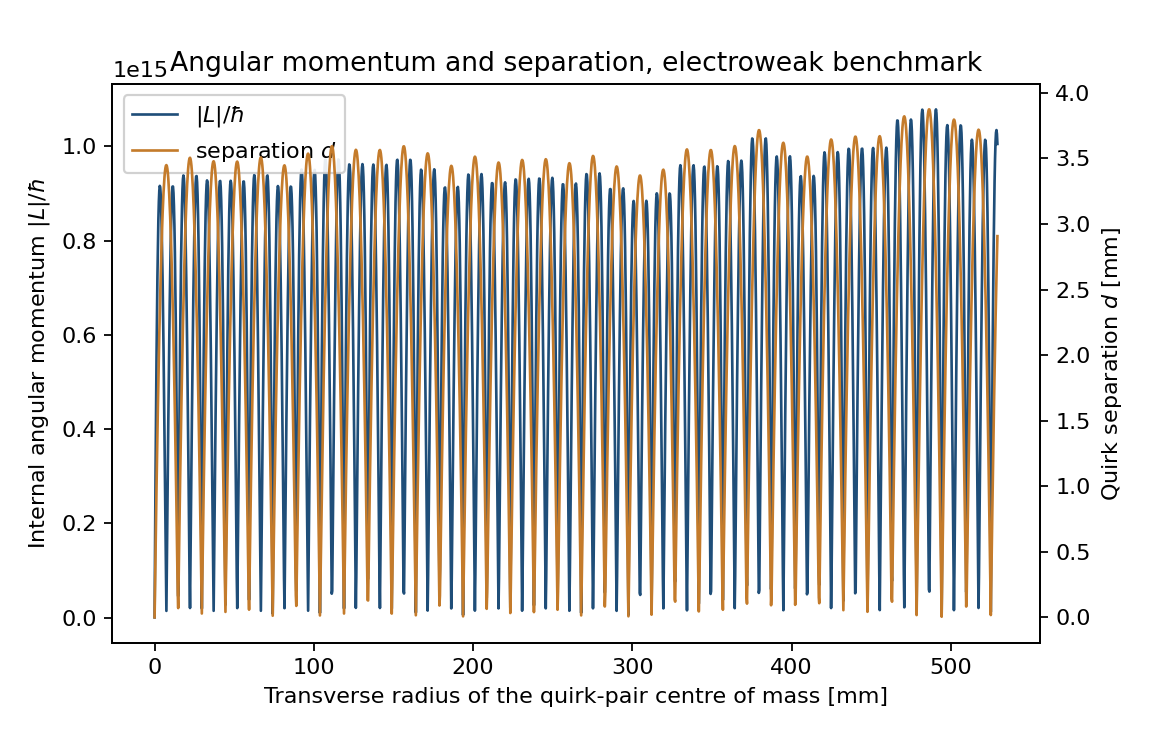
\includegraphics[width=\textwidth]{fig2_angular_momentum.png}
\caption{Internal angular momentum \(|L|/\hbar\) and quirk separation \(d\) versus the transverse radius of the pair centre of mass, for one electroweak event at \SI{800}{\GeV} and \SI{4}{\keV}.
On this trajectory \(|L|/\hbar\) reaches \(1.08\times 10^{15}\), and \(d\) oscillates between \SI{0.001}{\mm} and \SI{3.87}{\mm}.
This is the same pair of quantities as Figure~2 of the paper.}
\label{fig:l}
\end{figure}

\begin{figure}[H]
\centering
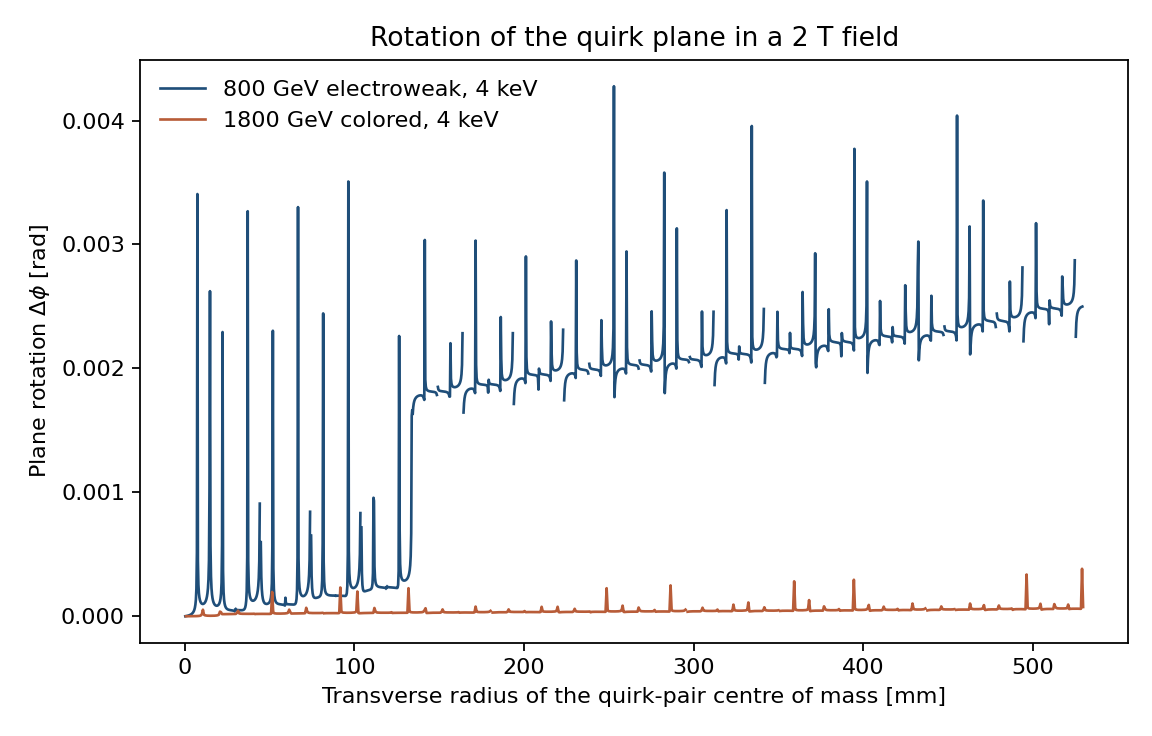
\includegraphics[width=\textwidth]{fig3_plane_rotation.png}
\caption{Angle \(\Delta\phi\) between the instantaneous quirk plane and the plane at the start of the trajectory.
The electroweak event reaches \(4.3\times 10^{-3}\,\mathrm{rad}\).
The colored event, at \SI{1800}{\GeV} and \SI{4}{\keV}, reaches \(3.8\times 10^{-4}\,\mathrm{rad}\).
As in Figure~3 of the paper, the rotation remains small compared with the tracker resolution.}
\label{fig:phi}
\end{figure}

\begin{figure}[H]
\centering
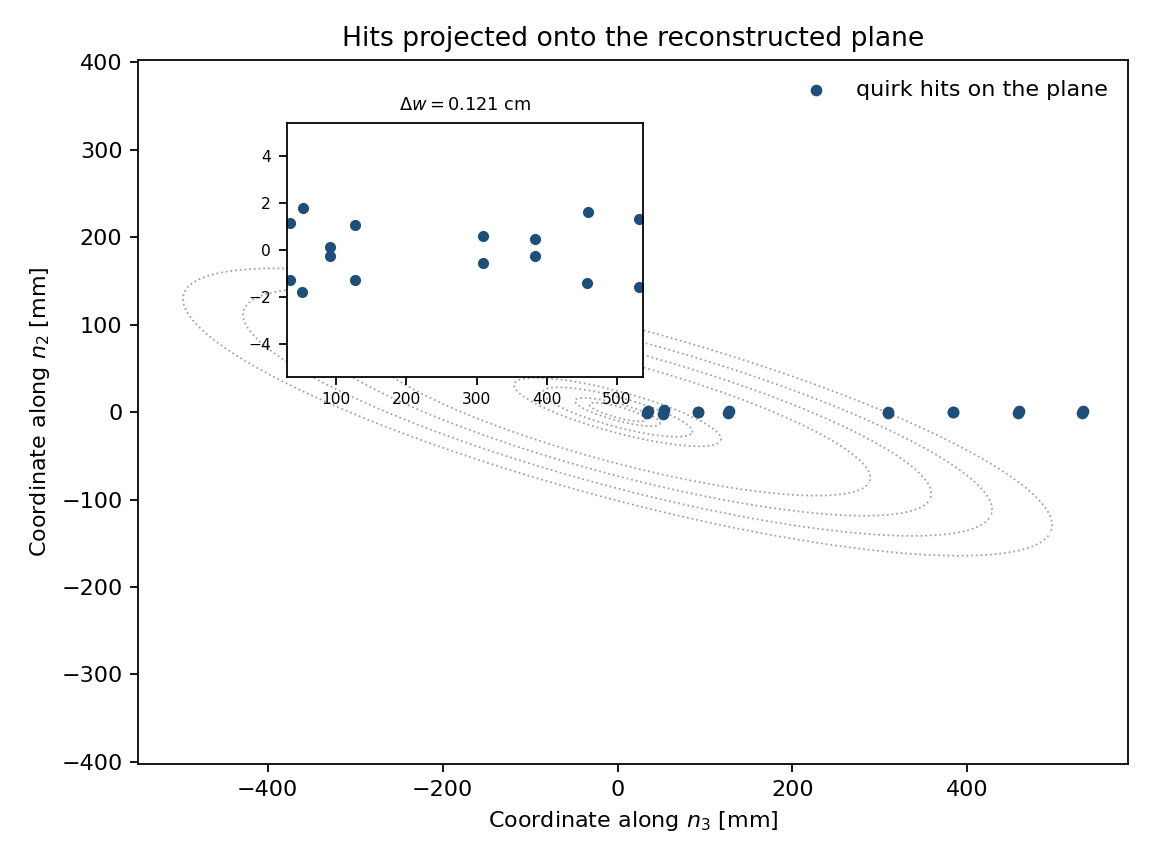
\includegraphics[width=0.92\textwidth]{fig4_plane_projection.png}
\caption{Hits of one electroweak event projected onto the reconstructed \((\boldsymbol{n}_3,\boldsymbol{n}_2)\) plane.
The dotted curves are the eight barrel layers.
The fit gives \(\Delta s = \SI{0.0027}{\cm}\) and \(\Delta w = \SI{0.121}{\cm}\), from 16 hits.
The inset shows the strip, as in Figure~4 of the paper.}
\label{fig:plane}
\end{figure}

\begin{figure}[H]
\centering
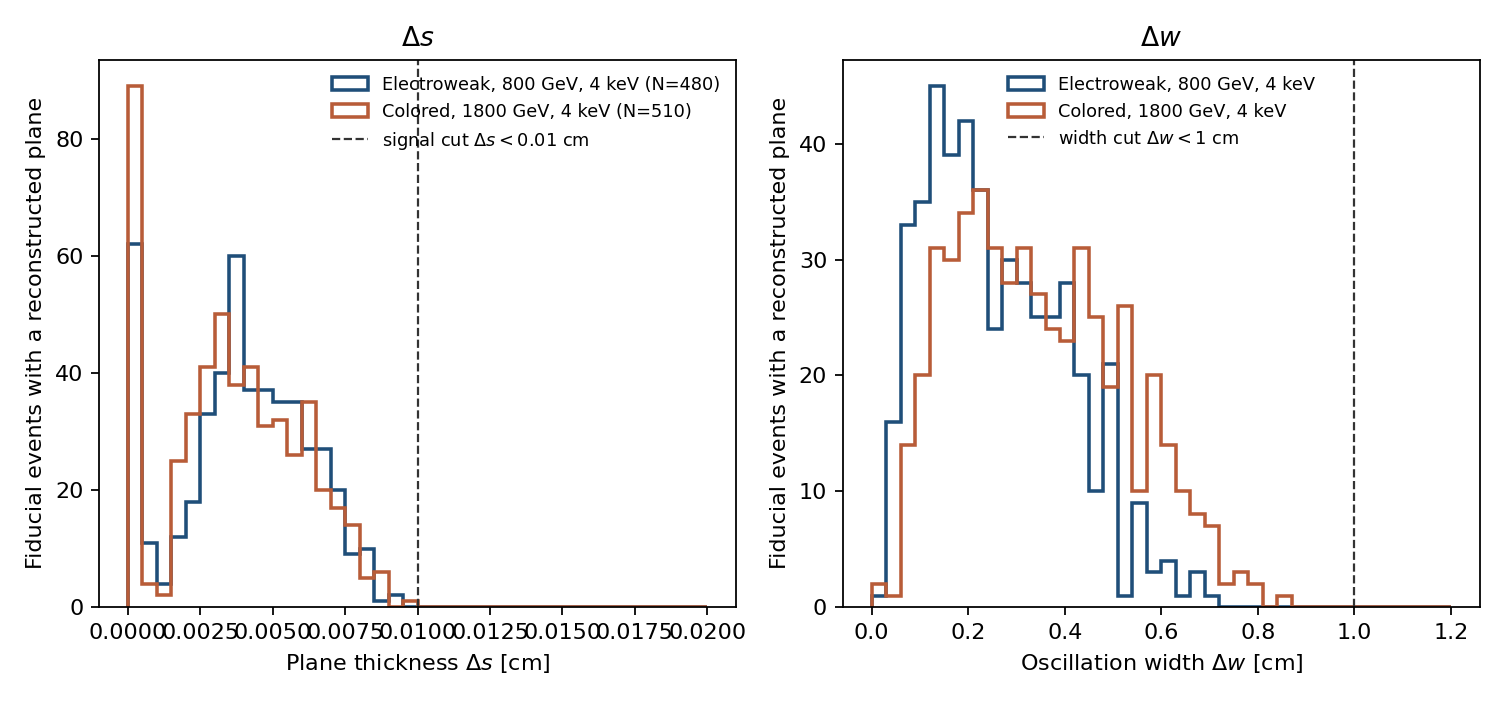
\includegraphics[width=\textwidth]{fig5_delta_s_delta_w.png}
\caption{Thickness \(\Delta s\) and width \(\Delta w\) for fiducial events in which the plane finder returned a plane, before the hit-pattern requirement.
The dashed line on the left is the signal cut \(\Delta s < \SI{0.01}{\cm}\).
The dashed line on the right is \(\Delta w < \SI{1}{\cm}\).
There are 480 electroweak events and 510 colored events in the histograms.
Figure~5 of the paper also shows the pileup and photon-conversion background, which was not generated in this run, and its colored curve is at \SI{2}{\keV} rather than \SI{4}{\keV}.}
\label{fig:widths}
\end{figure}

\end{document}
